\documentclass[paper=a4, fontsize=12pt]{scrreprt}
%fürs nächste mal nicht so große Abstände
\usepackage[left=2.5cm,right=2cm,top=1cm,bottom=1cm]{geometry}
\geometry{headheight=1cm, headsep=1.5cm, includehead}
\geometry{footskip=1.5cm ,includefoot}
\usepackage[ngerman]{babel}
\usepackage[
	colorlinks = true,
	linkcolor =,
	urlcolor  = blue,
	citecolor = black,
	anchorcolor = blue,
	hypertexnames=false
]{hyperref}
\usepackage{lineno}
\usepackage{csquotes}
\usepackage{enumitem}
\usepackage{caption}
\usepackage{booktabs}
\usepackage{graphicx} 
\usepackage[headsepline, footsepline, plainheadsepline=false, plainfootsepline=false, automark, autooneside=false, markcase=used]{scrlayer-scrpage}
\automark{chapter}
\pagestyle{scrheadings}
\usepackage{blindtext}
\usepackage[acronym,nopostdot]{glossaries}
\makeglossaries
\usepackage{tabularx}
\usepackage[table]{xcolor}
\usepackage{xcolor,colortbl}
\usepackage{makecell} %for bigger lines in table
\usepackage{multicol}
\usepackage{multirow}
\usepackage{changepage}
\usepackage{ragged2e}
\usepackage{amssymb}
\usepackage{amsfonts} % <- zusätzliche Mathesymbole
\usepackage{mathtools} % <- zusätzliche Mathesymbole
\usepackage{setspace} %Zeilenabstand
\usepackage{pgfplots} \pgfplotsset{compat=1.7}
\usepackage{todonotes}
\usepackage{makecell}
\usepackage{pdfpages}
\usepackage{numprint}
\npthousandsep{\,}
%%-----------------------------------------------------------------------------------
%% BibLaTex
\usepackage[backend=bibtex, style=numeric, sorting=none]{biblatex}
\addbibresource{quellen.bib}
\renewcommand*{\labelnamepunct}{\addcolon\addspace}     % Semikollon nach Autor
\renewcommand*{\newunitpunct}{\addsemicolon\space} 		% Trennzeichen Semikolon

%----------------------------------------------------------------------------------------
% 						Helping Commands
%
% \renewcommand{\arraystretch}{1.2} 	<- Tabelle strecken um 1.2 Punkte
% \rowcolors{1}{black!10}{black!1}		<- 
%

%Tabellenlinie
\newcommand\btrule[1]{\specialrule{#1}{0pt}{0pt}}
\newcolumntype{?}{!{\vrule width 1pt}}

%Tabellenheader White & Bold
\newcommand{\whitebf}[1]{\color{white}\textbf{#1}}

%deutsche Anführungszeichen (german quote)
\newcommand{\gequote}[1]{\glqq #1\grqq{}}

%url in footnotesize
\newcommand{\smallerurl}[1]{{\footnotesize\url{#1}}}

% Parttitle nutzbar machen
\let\Oldpart\part
\newcommand{\parttitle}{}
\renewcommand{\part}[1]{\Oldpart{#1}\renewcommand{\parttitle}{#1}}

%Auch bei chapter Header und Footer
\renewcommand*\chapterpagestyle{useheadings}

%Chapter Abstände
\renewcommand*\chapterheadstartvskip{\vspace*{-2.5\topskip}}
\renewcommand*\chapterheadendvskip{%
	\vspace*{1\baselineskip plus .1\baselineskip minus .167\baselineskip}}

\def\LayoutTextField#1#2{% label, field
	#2%
}
\renewcommand*{\DefaultOptionsofText}{print, bordercolor=black, borderstyle=U, backgroundcolor=blue!30}

\newcommand{\Todo}[1]{\todo[linecolor=red,backgroundcolor=red!25,bordercolor=red]{#1}}
\newcommand{\Info}[1]{\todo[linecolor=green,backgroundcolor=green!25,bordercolor=green]{#1}}

%\let\olditem\item
%\newcommand{\blueitem}{\color{blue}\olditem}
%\renewcommand{\item}{\color{black}\olditem}

%tabularx Gimmick
\newcolumntype{R}{>{\raggedleft\arraybackslash}X}
\newcolumntype{L}{>{\raggedright\arraybackslash}X}
\newcolumntype{C}{>{\centering\arraybackslash}X}

%----------------------------------------------------------------------------------------
%	Listings
%----------------------------------------------------------------------------------------
\usepackage{listings}
\usepackage{color}

\definecolor{mygreen}{rgb}{0,0.6,0}
\definecolor{mygray}{rgb}{0.5,0.5,0.5}
\definecolor{mymauve}{rgb}{0.58,0,0.82}

\definecolor{black}{rgb}{0,0,0}
\definecolor{white}{rgb}{1,1,1}
\definecolor{magicmint}{rgb}{0.67, 0.94, 0.82}



\lstset{ 
	backgroundcolor=\color{white},   % choose the background color; you must add \usepackage{color} or \usepackage{xcolor}; should come as last argument
	basicstyle=\footnotesize,        % the size of the fonts that are used for the code
	breakatwhitespace=false,         % sets if automatic breaks should only happen at whitespace
	breaklines=true,                 % sets automatic line breaking
	captionpos=t,                    % sets the caption-position to bottom
	commentstyle=\color{gray},    % comment style
	deletekeywords={...},            % if you want to delete keywords from the given language
	escapeinside={\%*}{*)},          % if you want to add LaTeX within your code
	extendedchars=true,              % lets you use non-ASCII characters; for 8-bits encodings only, does not work with UTF-8
	firstnumber=1,                % start line enumeration with line 1000
	frame=single,	                   % adds a frame around the code
	keepspaces=true,                 % keeps spaces in text, useful for keeping indentation of code (possibly needs columns=flexible)
	keywordstyle=\color{blue},       % keyword style
	language=Octave,                 % the language of the code
	morekeywords={*,...},            % if you want to add more keywords to the set
	numbers=left,                    % where to put the line-numbers; possible values are (none, left, right)
	numbersep=8pt,                   % how far the line-numbers are from the code
	numberstyle=\footnotesize\color{mygray}, % the style that is used for the line-numbers
	rulecolor=\color{black},         % if not set, the frame-color may be changed on line-breaks within not-black text (e.g. comments (green here))
	showspaces=false,                % show spaces everywhere adding particular underscores; it overrides 'showstringspaces'
	showstringspaces=false,          % underline spaces within strings only
	showtabs=false,                  % show tabs within strings adding particular underscores
	stepnumber=1,                    % the step between two line-numbers. If it's 1, each line will be numbered
	stringstyle=\color{mymauve},     % string literal style
	tabsize=2,	                   % sets default tabsize to 2 spaces
	title=\lstname                   % show the filename of files included with \lstinputlisting; also try caption instead of title
}
\setlength\parindent{0pt}

%----------------------------------------------------------------------------------------
% Glossary
\setglossarysection{section}
\newglossarystyle{tabX3col}{
	\renewenvironment{theglossary}%
	{\renewcommand{\arraystretch}{1.5}\tabular{p{.2\linewidth} p{.55\linewidth} >{\raggedleft\arraybackslash}p{.15\linewidth}}}%
	{\endtabular}%
	\renewcommand*{\glossaryheader}{\textbf{Bezeichnung} & \textbf{Erklärung} & \textbf{Seitenzahlen}\\[5px]}%
	\renewcommand*{\glsgroupheading}[1]{}%
	\renewcommand*{\glsgroupskip}{}%
	\renewcommand{\glossentry}[2]{%
		\glossentryname{##1} & \glossentrydesc{##1}\hfill & ##2\\\hline%
	}%
	\renewcommand*{\subglossentry}[3]{}
}
% Glossaryentry
\newglossaryentry{ohdmconverter}{
	name=OHDMConverter,
	description={Javabasierte Applikation, die alle Portierungen der verschiedenen Datenbankschemata und Skripte enthält}	
}
\newglossaryentry{ohm}{
	name=OHM,
	description={HTW Berlin interne Bezeichnung für den physischen Server für das Open Historical Data Map Projekt}	
}

\newglossaryentry{inter}{
	name=Intermediate,
	description={Benamung für das Datenbankschema, das für die Konvertierung von einer OpenStreetMap Datei in eine Zwischendatenbank genutzt wird}
}

\newglossaryentry{osm2inter}{
	name=osm2inter,
	description={Abkürzung für die Konvertierungsmethode von einer OpenStreetMap Datei in eine Zwischendatenbank (Intermediate Datenbank)}
}

% Acronyms
\newacronym{gui}{GUI}{Graphical User Interface}
\newacronym{ohdm}{OHDM}{Open Historical Data Map}
\newacronym{dbms}{DBMS}{Database Management System}
\newacronym{db}{DB}{Datenbank}
\newacronym{osm}{OSM}{OpenStreetMap}
\newacronym{pbf}{PBF}{Protocolbuffer Binary Format}
\newacronym{htw}{HTW}{Hochschule für Technik und Wirtschaft}
%----------------------------------------------------------------------------------------
\newcommand{\printTitle}{Bericht über die Praktikumstätigkeit}

\begin{document}
	\pagestyle{empty}
\clearmainofpairofpagestyles
\begin{figure}
	\centering
	\includegraphics{img/htw_logo.jpg}
	\vspace{60pt}
\end{figure}
\begin{center}
	\huge{Bericht über die Praktikumstätigkeit}\\
	\begin{large}
		Implementierung einen neuen Prototyps des OHDMConverters\\[1cm]
		\textbf{an der HTW Berlin}\\[0.4cm]
		Fachbereich 4 - Informatik, Kommunikation und Wirtschaft,\\
		Studiengang Angewandte Informatik\\[4cm]
		\textbf{Zeitraum des Fachpraktikums}\\
		14.02.2022 - 14.05.2022\\[1.5cm]
	\end{large}
	
	\begin{normalsize}
		\begin{tabularx}{\linewidth}{R X}
			\textbf{Vorname, Name} & Stefan Sadewasser\\
			\textbf{Matrikelnummer} & 568158\\
			\textbf{Studiengang, Fachbereich} & Angewandte Informatik, Fachbereich 4\\
			\textbf{E-Mail} & \href{mailto:stefan.sadewasser@student.HTW-Berlin.de}{stefan.sadewasser@student.HTW-Berlin.de}
		\end{tabularx}
	\end{normalsize}\vspace{1cm}
\end{center} 
\newpage

\addtocontents{toc}{\protect\thispagestyle{empty}}
\setcounter{tocdepth}{1}
%\chapter is level 0
%\section is level 1
%\subsection is level 2
%\subsubsection is level 3
%\paragraph is level 4
%\subparagraph is level 5
\tableofcontents
\newpage

{\Huge \textbf{Abk\"urzungsverzeichnis}}\\
\begin{acronym}
	\acro{GUI}{Graphical User Interface}
	\acro{OHDM}{Open Historical Data Map}
	\acro{DBMS}{Database Management System}
	\acro{OSM}{OpenStreetMap}
	\acro{PBF}{Protocolbuffer Binary Format}
\end{acronym}
\clearpage
	
	\newpage \setheadsepline{.5px} \setfootsepline{.5px}
\setcounter{page}{1}
\ihead{} \chead{} \ohead{\headmark}
\ifoot{} \cfoot{\pagemark} \ofoot{}
\part{Praktikumsplan, Datenbank, javabasierte Konvertierung}
\chapter{Praktikum}
\section{Arbeitsauftrag}
Im Rahmen des Praktikums sollte ein Linux-Server vor ein Kartenprojekt neu
aufgesetzt werden. In Zusammenarbeit mit den Administratoren vor Ort musste ein
PostGIS-Datenbankserver aufgesetzt werden. Danach sollte eine DBs aufgesetzt werden, die in Summe ca. 1
TByte Daten verwalten kann. Das Füllen der DBs würde über vorhandene Tools erfolgen. Die zusätzliche Aufgabe war es Studierende zu unterstützt, die an der Weiterentwicklung dieser Tools arbeiten.

Die Arbeit sollte wie folgt aufgeteilt werden:
\begin{enumerate}
	\item Dokumentation und Aufsetzen der Testumgebung
	\begin{enumerate}
		\item Dokumentation einer Installationsanleitung für die Benutzung des \newline OHDMConverters zur Importierung von \ac{OSM} Daten
		\item Dokumentation der Aufsetzung einer Testumgebung
		\item Dokumentation wie in 1a für Windows und MacOS Systeme
	\end{enumerate}
	\item Wiederaufsetzen des physischen OHM Servers
	\begin{enumerate}
		\item Aufsetzen 2 separater Datenbankserver auf dem physischen OHM Server
		\item Importierung des planet.osm Datensatzes im Produktivdatenbankserver
		\item Formulierung eines Cron-Jobs zur Automatisierung
		\item Importierung von \ac{OSM} Daten von Deutschland im Integrationsdatenbankserver
	\end{enumerate}
\end{enumerate}

\section{Planung}
Die Aufteilung wurde in separierten Arbeitspaketen festgehalten, welche dann im Planungskalender für ein oder zwei Kalenderwochen Bearbeitungszeit eingetragen wurden.\\
\begin{tabularx}{\linewidth}{|X|X|X|X|X|X|X|X|X|X|X|X|X|X|X|}
	\hline
	KW & 7 & 8 & 9 & 10 & 11 & 12 & 13 & 14 & 15 & 16 & 17 & 18 & 19 & 20\\\hline
	\multicolumn{2}{c}{\cellcolor{blue!25}AP 1a} &&&&&&&&&&&&&\\\hline
	& \multicolumn{2}{c}{\cellcolor{blue!25}AP 1b} &&&&&&&&&&&&\\\hline
	&&& \multicolumn{2}{c}{\cellcolor{blue!25}AP 2a} &&&&&&&&&&\\\hline
	&&&& \multicolumn{2}{c}{\cellcolor{blue!25}AP 2b} &&&&&&&&&\\\hline
	&&&&&& \multicolumn{2}{c}{\cellcolor{blue!25}AP 1c} &&&&&&&\\\hline
	&&&&&&&& \multicolumn{2}{c}{\cellcolor{blue!25}AP 2c} &&&&&\\\hline
	&&&&&&&&& \multicolumn{2}{c}{\cellcolor{blue!25}AP 2d} &&&&\\\hline
\end{tabularx}

\chapter{Datenbankserver}
Der Datenbankserver sollte mit 2 separaten PostGIS Datenbanken erstellt werden. Die Erstellung und Einrichtung des Servers selbst geschah in enger Zusammenarbeit mit dem \\
Laboringenieur Axel Wagner.\\
Der OHM Server wurde mit einem \href{https://releases.ubuntu.com/20.04/}{\underline{Ubuntu 20.04}} in englischer Sprache und ohne \ac{GUI} eingerichtet.\\
Des Weiteren wurden auf dem Server mehrere administrative Tools installiert, welche den Mitarbeitern beziehungsweise Laboringenieuren die Arbeit mit den Servern erleichtern.
\begin{enumerate}[label=\textbf{\arabic*.}]
	\item \textbf{aptitude}\\ist eine Erweiterung der Paketverwaltung APT, aber im Gegensatz zu apt-get führt aptitude über Änderungen der installierten Pakete \gequote{genauer} Buch, so dass nicht mehr benötigte Pakete automatisch erkannt und deinstalliert werden. Die Installationsgeschichte wird in ein Log geschrieben, wodurch später angezeigt werden kann, wann oder warum ein Paket installiert wurde.
	\item \textbf{openssh-server}\\Die OpenSSH-Serverkomponente sshd wartet ständig auf Client-Verbindungen von einem der Client-Tools. Wenn eine Verbindungsanforderung auftritt, baut sshd die richtige Verbindung auf, je nachdem, welches Client-Tool die Verbindung herstellt. Wenn sich der entfernte Computer beispielsweise mit der ssh-Client-Anwendung verbindet, baut der OpenSSH-Server nach der Authentifizierung eine Fernsteuerungssitzung auf. Wenn ein entfernter Benutzer eine Verbindung zu einem OpenSSH-Server mit scp herstellt, initiiert der OpenSSH-Server-Daemon nach der Authentifizierung eine sichere Kopie von Dateien zwischen dem Server und dem Client.
	\item \textbf{net-tools}\\Eine Sammlung von Programmen, die den Basissatz der NET-3-Netzwerkdistribution für das Linux-Betriebssystem bilden. Dieses Paket enthält arp, hostname, ifconfig, ipmaddr, iptunnel, mii-tool, nameif, netstat, plipconfig, rarp, route und slattach.
	\item \textbf{git}\\ist ein dezentrales Versionsverwaltungssystem.
	\item \textbf{nullmailer}\\ist ein reiner Weiterleitungs-MTA (Mail Transfer Agent). Das bedeutet, dass alle auf einem System eingehenden E-Mails an einen konfigurierten externen Mailserver weitergeleitet werden. Dies kann nützlich sein, wenn die Installation eines lokalen E-Mail-Servers nicht erwünscht oder nicht wirklich sinnvoll ist, aber zumindest die System-E-Mails müssen irgendwo hin weitergeleitet werden.
	\item \textbf{logwatch}\\ist ein in Perl geschriebenes Tool zur Analyse von Logdateien. Es soll Systemadministratoren helfen, die Übersicht über alle Vorgänge auf einem Serversystem zu behalten. Logwatch durchsucht die Logdateien des Systems und generiert eine Kurzfassung daraus, deren Gestaltung individuell konfiguriert werden kann. Diese kann dann entweder als Datei weiterverarbeitet oder zum Versenden an einen Mailserver weitergereicht werden.
	\item \textbf{apticron}\\ist ein kleines Shellskript zur automatischen Benachrichtigung über Paket-Updates per E-Mail.
	\item \textbf{fail2ban}\\ist ein Set aus Client, Server und Konfigurationsdateien, welches Logdateien überwacht, dort nach vordefinierten Mustern sucht und nach diesen temporär IP-Adressen sperrt.
\end{enumerate}\vspace{1cm}

Der OHM Server ist wie auch das \ac{OHDM} Projekt eine HTW Berlin Projekt, somit musst auch die Erreichbarkeit des Server aus dem HTW Netz gewährleistet werden. Dies wurde mit einem bash Script realisiert, das \textit{iptables} Einträge zur Port/IP Freigabe enthält.\\

Das \ac{OHDM} Projekt benutzt als \ac{DBMS} PostgreSQL mit PostGIS als Erweiterung.\\
Der erste Schritt, ist die Installierung von PostgreSQL. Dieser lässt sich auf Ubuntu 20.04 wie in \autoref{lst:install-postgresql} installieren.
\begin{lstlisting}[language=bash,caption={Installation PostgreSQL},label={lst:install-postgresql}]
sudo sh -c 'echo "deb http://apt.postgresql.org/pub/repos/apt $(lsb_release -cs)-pgdg main" > /etc/apt/sources.list.d/pgdg.list'
wget --quiet -O - https://www.postgresql.org/media/keys/ACCC4CF8.asc | sudo apt-key add -
sudo apt-get update
sudo apt-get -y install postgresql-14
# from 2022-02-24
\end{lstlisting}
Im Anschluss kann PostGIS als eine räumliche Datenbankerweiterung für PostgreSQL (siehe \autoref{lst:install-postgis}) installiert werden.
\begin{lstlisting}[language=bash,caption={Installation PostGIS},label={lst:install-postgis}]
sudo apt-get install postgresql-14-postgis-3
sudo apt-get install postgresql-14-postgis-3-scripts
\end{lstlisting}

Während der Installationen sollte standardmäßig ein PostgreSQL Cluster\cite{postgresql-cluster} erstellt werden, welches folgende Daten besitzt:\\[0.5cm]
\begin{tabular}{r l}
	Servername: & localhost\\
	Port: & 5432\\
	Clustername: & main\\
	Datenbankbenutzer & postgres\\
	Standarddatenbank & postgres\\
	Datenbasis & \lstinline[language=bash]|/var/lib/postgresql/14/main|\\
	Datenbank log Datei & \lstinline[language=bash]|/var/log/postgresql/postgresql-14-main.log|\\
	Pfad zu den Konfigurationen & \lstinline[language=bash]|/etc/postgresql/14/main/|\\
\end{tabular}

\newpage
\section{Multiple Datenbanken in PostgreSQL}
Mit PostgreSQL ist es möglich mehrere Datenbanken parallel laufen zu lassen.\\
Anhand des Arbeitspaketes sollten 2 zusätzliche Cluster auf dem OHM Server entstehen. Hierfür wurden bestehende beziehungsweise mitinstallierte Tools verwendet.

\subsection{Cluster erzeugen}\label{subsec:create-cluster}
Zur Erzeugung eines neuen PostgreSQL Clusters wird der Befehl in \autoref{lst:create-cluster} verwendet. Für eine detaillierte Beschreibung der Clusterdaten dient \autoref{lst:create-cluster} Zeile \ref{ln:create-cluster} als Vorlage.\\ Weitere Überlegungen dazu in \autoref{ch:clustering}.
\begin{lstlisting}[language=bash,caption={Erzeugung eines PostgreSQL Clusters},label={lst:create-cluster}]
sudo pg_createcluster [postgresql_version_number] [clustername] -p [port]
# Beispiel mit integration
sudo pg_createcluster 14 integration -p 5433\%*\label{ln:create-cluster}*)
\end{lstlisting}

Durch die Verwendung des Befehls aus \autoref{lst:create-cluster} werden die Clusterdaten wie folgt erzeugt:\\[0.5cm]
\begin{tabular}{r l}
	Servername: & localhost\\
	Port: & 5432\\
	Clustername: & integration\\
	Datenbankbenutzer & postgres\\
	Standarddatenbank & postgres\\
	Datenbasis & \lstinline[language=bash]|/var/lib/postgresql/14/integration|\\
	Datenbank log Datei & \lstinline[language=bash]|/var/log/postgresql/postgresql-14-integration.log|\\
	Pfad zu den Konfigurationen & \lstinline[language=bash]|/etc/postgresql/14/integration|\\
\end{tabular}\vspace{0.5cm}

Weitere Informationen unter:\\ \url{http://manpages.ubuntu.com/manpages/trusty/man8/pg_createcluster.8.html}\\[0.5cm]

\subsection{Cluster steuern}
Ein \lstinline[language=bash]|start|/\lstinline[language=bash]|stop| oder \lstinline[language=bash]|restart| lässt sich nun mit dem Befehl in \autoref{lst:ctlcluster} realisieren.
\begin{lstlisting}[language=bash,caption={Steuerung des Clusters},label={lst:ctlcluster}]
sudo pg_ctlcluster [postgresql_version_number] [clustername] [start|stop|restart]
# Beispiel mit integration
sudo pg_ctlcluster 14 integration [start|stop|restart]
\end{lstlisting}
Auch hierzu gibt es weitere Informationen, die unter:\\ \url{http://manpages.ubuntu.com/manpages/trusty/man8/pg_ctlcluster.8.html}\\
eingesehen werden können.\newpage

\subsection{Cluster als Service registrieren}
Eine Integration des erstellten Clusters als Service ist in \autoref{lst:cluster-enable} einzusehen. Dies wird benötigt um auch nach einem Server Neustart gewährleisten zu können das der Datenbank Server dieses Clusters erreichbar ist.
\begin{lstlisting}[language=bash,caption={Registierung des Clusters als System Service},label={lst:cluster-enable}]
sudo systemctl enable postgresql@[postgresql_version_number]-[clustername].service
# Beispiel mit integration
sudo systemctl enable postgresql@14-integration.service
\end{lstlisting}

\section{Datenbank Fernzugriff}
Für eine Freigabe des Zugriffs auf die Datenbank von anderen Adressen als den \lstinline|localhost| muss nicht nur der physische Server mit entsprechenden Freigaben eingestellt werden, sondern auch die Datenbank selbst.\\
Hierfür müssen die Konfigurationsdateien \textit{postgresql.conf} und \textit{pg\_hba.conf} der Datenbank angepasst werden. Diese befinden sich im Pfad: \lstinline|/etc/postgresql/[version_number]/[clustername]/| beziehungsweise am Beispiel \lstinline|integration|: \lstinline|/etc/postgresql/14/integration| (vgl. \autoref{subsec:create-cluster})

\subsection{postgresql.conf}
In der Datenbankkonfigurationsdatei können einige Anpassungen vorgenommen werden. In diesem Beispiel wird sich auf die Anpassung der Abgehörten IP Adressen beschränkt.\\
in den Grundeinstellungen ist ein PostgreSQL Datenbank Server so eingestellt das ein Zugriff auf die Daten nur Lokal möglich ist. Für die Möglichkeit eines Fernzugriffs auf die Daten muss der Eintrag (siehe \autoref{lst:postgrsql-conf}) geändert werden. Wie in den Kommentaren ersichtlich kann dabei auf 2 Varianten zurückgegriffen werden.
\begin{enumerate}
	\item Freigabe einer Liste von IP Adressen die durch Komma separiert sind oder
	\item Freigabe aller IP Adressen durch Benutzung \gequote{*}
\end{enumerate}
Die 2. Variante sollte die fehlerfreie Freigabe von IP Adressen in den Firewall Einstellungen enthalten. Damit keine Sicherheitskonzepte verletzt werden.

\begin{lstlisting}[language=bash,caption={postgresql.conf Ausschnitt},label={lst:postgrsql-conf},commentstyle=\color{black}]
# - Connection Settings -

#listen_addresses = 'localhost'		# what IP address(es) to listen on;
# comma-separated list of addresses;
# defaults to 'localhost'; use '*' for all
# (change requires restart)
\end{lstlisting}

\newpage
\subsection{pg\_hba.conf}
Die Einstellungen der Authentifizierungsmethode werden in der Datenbankkonfigurationsdatei \textit{pg\_hba.conf} definiert. In \autoref{lst:pg-hba-conf} ist ein Ausschnitt einer solchen Datei auf einem Ubuntu 20.04 zu sehen. Diese definiert zum Beispiel in Zeile \ref{ln:postgres-without-password} eine Peer Authentifikation des Systembenutzers \textit{postgres}.\\
Bei der Peer-Authentifizierungsmethode wird der Betriebssystem-Benutzername des Clients vom Kernel abgerufen und als zulässiger Datenbank-Benutzername verwendet (mit optionaler Zuordnung der Benutzernamen). Diese Methode wird nur bei lokalen Verbindungen unterstützt.(vgl. \autocite{peer-authentification})
\begin{lstlisting}[caption={pg\_hba.conf Ausschnitt},label={lst:pg-hba-conf},deletekeywords={all}]
# Database administrative login by Unix domain socket
local		all				 		postgres	       					     peer\%*\label{ln:postgres-without-password}*)

# TYPE  DATABASE    	USER        ADDRESS             METHOD

# "local" is for Unix domain socket connections only
local   all         	all                             peer
# IPv4 local connections:
host    all         	all         127.0.0.1/32        scram-sha-256
# IPv6 local connections:
host    all         	all         ::1/128             scram-sha-256
# Allow replication connections from localhost, by a user with the
# replication privilege.
local   replication 	all                             peer
host    replication 	all         127.0.0.1/32        scram-sha-256
host    replication 	all         ::1/128             scram-sha-256
\end{lstlisting}

\chapter{Konvertierung}
\section{OHDMConverter Java}
Der javabasierte OHDMConverter diente als Projekthilfsprogramm um alle Importierungen oder Konvertierungen einer Datei/Schema in ein anderes zu realisieren.\\
\textit{Annahme:} Da der OHDMConverter bis zum Beginn des Praktikums \gequote{nur} mit kleineren oder Testdatensätzen getestet und validiert wurde, konnten einige Fehler nicht gefunden werden.

\subsection{Importierung der planet.osm Datei}
Die Hauptaufgabe war es das planet.osm File in die PostgreSQL Datenbank zu importieren. Die Vorbereitung dieser Importierung musste mit größter Sorgfalt bearbeitet werden, um:
\begin{itemize}
	\item den fehlerfreien Ablauf zu gewährleisten,
	\item die Auslastung des physischen Servers so minimal wie möglich zu beschränken und
	\item Sicherheitskonzepte des physischen und des Datenbankservers einzuhalten.
\end{itemize}
Darüber hinaus musste auf die Größe der Datei berücksichtigt werden. Das heißt alle Tests fanden mit kleineren Dateien statt.

\begin{table}[h]
	\caption{Daten der planet.osm Datei}
	\renewcommand{\arraystretch}{1.5}
	\begin{tabularx}{\linewidth}{|C|C|}\hline
		Eigenschaft & Wert\\\btrule{1.2pt}
		Größe \ac{OSM} Datei & 115 GB\\\hline
		Größe der \ac{PBF}\cite{pbf} Datei & 63 GB \\\hline
		Anzahl Nodes in der Datenbank\cite{osm-taginfo} & \numprint{7663759219}\\\hline
		Anzahl Ways in der Datenbank\cite{osm-taginfo} & \numprint{856401369}\\\hline
		Anzahl Relations in der Datenbank\cite{osm-taginfo} & \numprint{9879181}\\\hline
	\end{tabularx}
	\caption*{Daten vom: 2022-05-03 23:59 UTC}
\end{table}

\newpage
\subsection{Fehlverhalten bei der Importierung}\label{subsec:error}
\subsubsection{admin\_level}
Der Schlüssel admin\_level=* beschreibt die Verwaltungsebene eines Merkmals innerhalb einer Regierungshierarchie. Er wird hauptsächlich für die Grenzen territorialer politischer Einheiten (z. B. Land, Staat, Gemeinde) zusammen mit boundary=administrative verwendet. Aufgrund kultureller und politischer Unterschiede entsprechen die Verwaltungsebenen verschiedener Länder nur annähernd einander.(vgl. \cite{osm:admin-level})

Von \ac{OSM} ist der Wert dieses Schlüssels als numerischer Wert zu speichern. Im \\OHDMConverter wurde auch von dieser Aussage ausgegangen, sodass für den Wert in Java ein Integer Wert angelegt wird und der Bedingung: Sollte der Wert nicht gelesen werden können wird das \ac{OSM} Objekt verworfen.\\
Der Folgefehler daraus ist, dass alle \ac{OSM} Objekte, die mit einem nicht numerischen Wert für den Schlüssel: \textit{admin\_level} eingetragen sind, nicht gelesen werden. Leider gibt es sehr viele dieser Objekte die für andere \ac{OSM} Objekte wichtig sind, sodass im Umkehrschluss Objekt zu dem das Objekt gehört nicht mehr darstellbar sind beziehungsweise einen fehlerhaften Querverweis haben.

\subsubsection{Abbruch}
Die Importierung der \ac{OSM} Datei in die PostgreSQL Datenbank wurde nicht vollständig ausgeführt. Anhand der log Dateien konnte ein Aussage zur Menge der nicht betrachteten \ac{OSM} Objekte und einem weiteren Fehler getroffen werden. Die beiden letzten Zeilen des logs von osm2inter, allerdings für die Dokumentation aufbereitet, kann in \autoref{lst:germany-osm2inter.log} eingesehen werden.
\begin{lstlisting}[language={},caption={Letzte zwei Zeilen des logs der Importierung von osm2inter},label={lst:germany-osm2inter.log}]
nodes: 7,505,830,920 
ways: 836,886,605 
relations: 2,382,475 
elapsed time:  9 : 5 : 58 : 30
throwable caught in startElement: 
java.lang.StringIndexOutOfBoundsException: 
begin 1, end 0, length 1
\end{lstlisting}

Zum Zeitpunkt der Importierung waren laut:\\ \url{https://taginfo.openstreetmap.org/reports/database_statistics}\\
\numprint{7565505545} Nodes, \numprint{844325562} Ways und \numprint{9742774} Relations in der planet.osm Datei enthalten. Somit fehlten der Datenbank:\\[0.5cm]
\begin{tabular}{r<{ kurz} r<{, das entspricht} r l}
	\numprint{60000000} & 60 Mio & 0,8\%& Nodes\\
	\numprint{8000000} & 8 Mio & 0,9\%& Ways\\
	\numprint{7000000} & 7 Mio &75,5\%& Relations	
\end{tabular}

\newpage
\section{Erkenntnis}
Aufgrund der gravierenden Fehler (vgl. \autoref{subsec:error}) im javabasierten OHDMConverter wurde die Lösung als Java Applikation verworfen. Dies geschah in Rücksprache mit dem Projektleiter Prof. Dr.-Ing. Thomas Schwotzer, welcher die Grundlegende Idee \ac{OSM} Daten in die \ac{OHDM} Datenbank zu importieren, als reines PsotgreSQL Projekt umsetzten wollte.\\
Das \ac{OHDM} Projekt beziehungsweise der OHDMConverter als Java Applikation läuft bereits seit einigen Jahren kann aber mit den aktuellen Mitteln nicht stabil genug implementiert werden (auch in absehbarer Zeit nicht).\\

Somit wurde die Projektidee neu definiert.
	\part{\gls{ohdmconverter} als PostgreSQL Projekt}
\chapter{Projektidee}
Die Grundidee von \gls{ohdm} ist immer noch die selbe, kurz es sollen \gls{osm} Daten um die Dimension Zeit erweitert werden. Auch bleiben die bestehenden Datenbankschemata gleich. Die größte Änderung ist die Implementierung.

\section{osm2inter}
Für den Import von \gls{osm} Dateien soll ein bestehendes Tool \gequote{\gls{osm2pgsql}}\cite{osm2pgsql} verwendet werden. \gls{osm2pgsql}\cite{osm2pgsql} ist dafür ausgelegt \gls{osm} Daten in eine PostGIS Datenbank zu importieren.

\begin{figure}[h]
	\caption{Entity Relationship Diagramm der \gls{inter} Datenbank}
	\label{fig:erd-inter}
	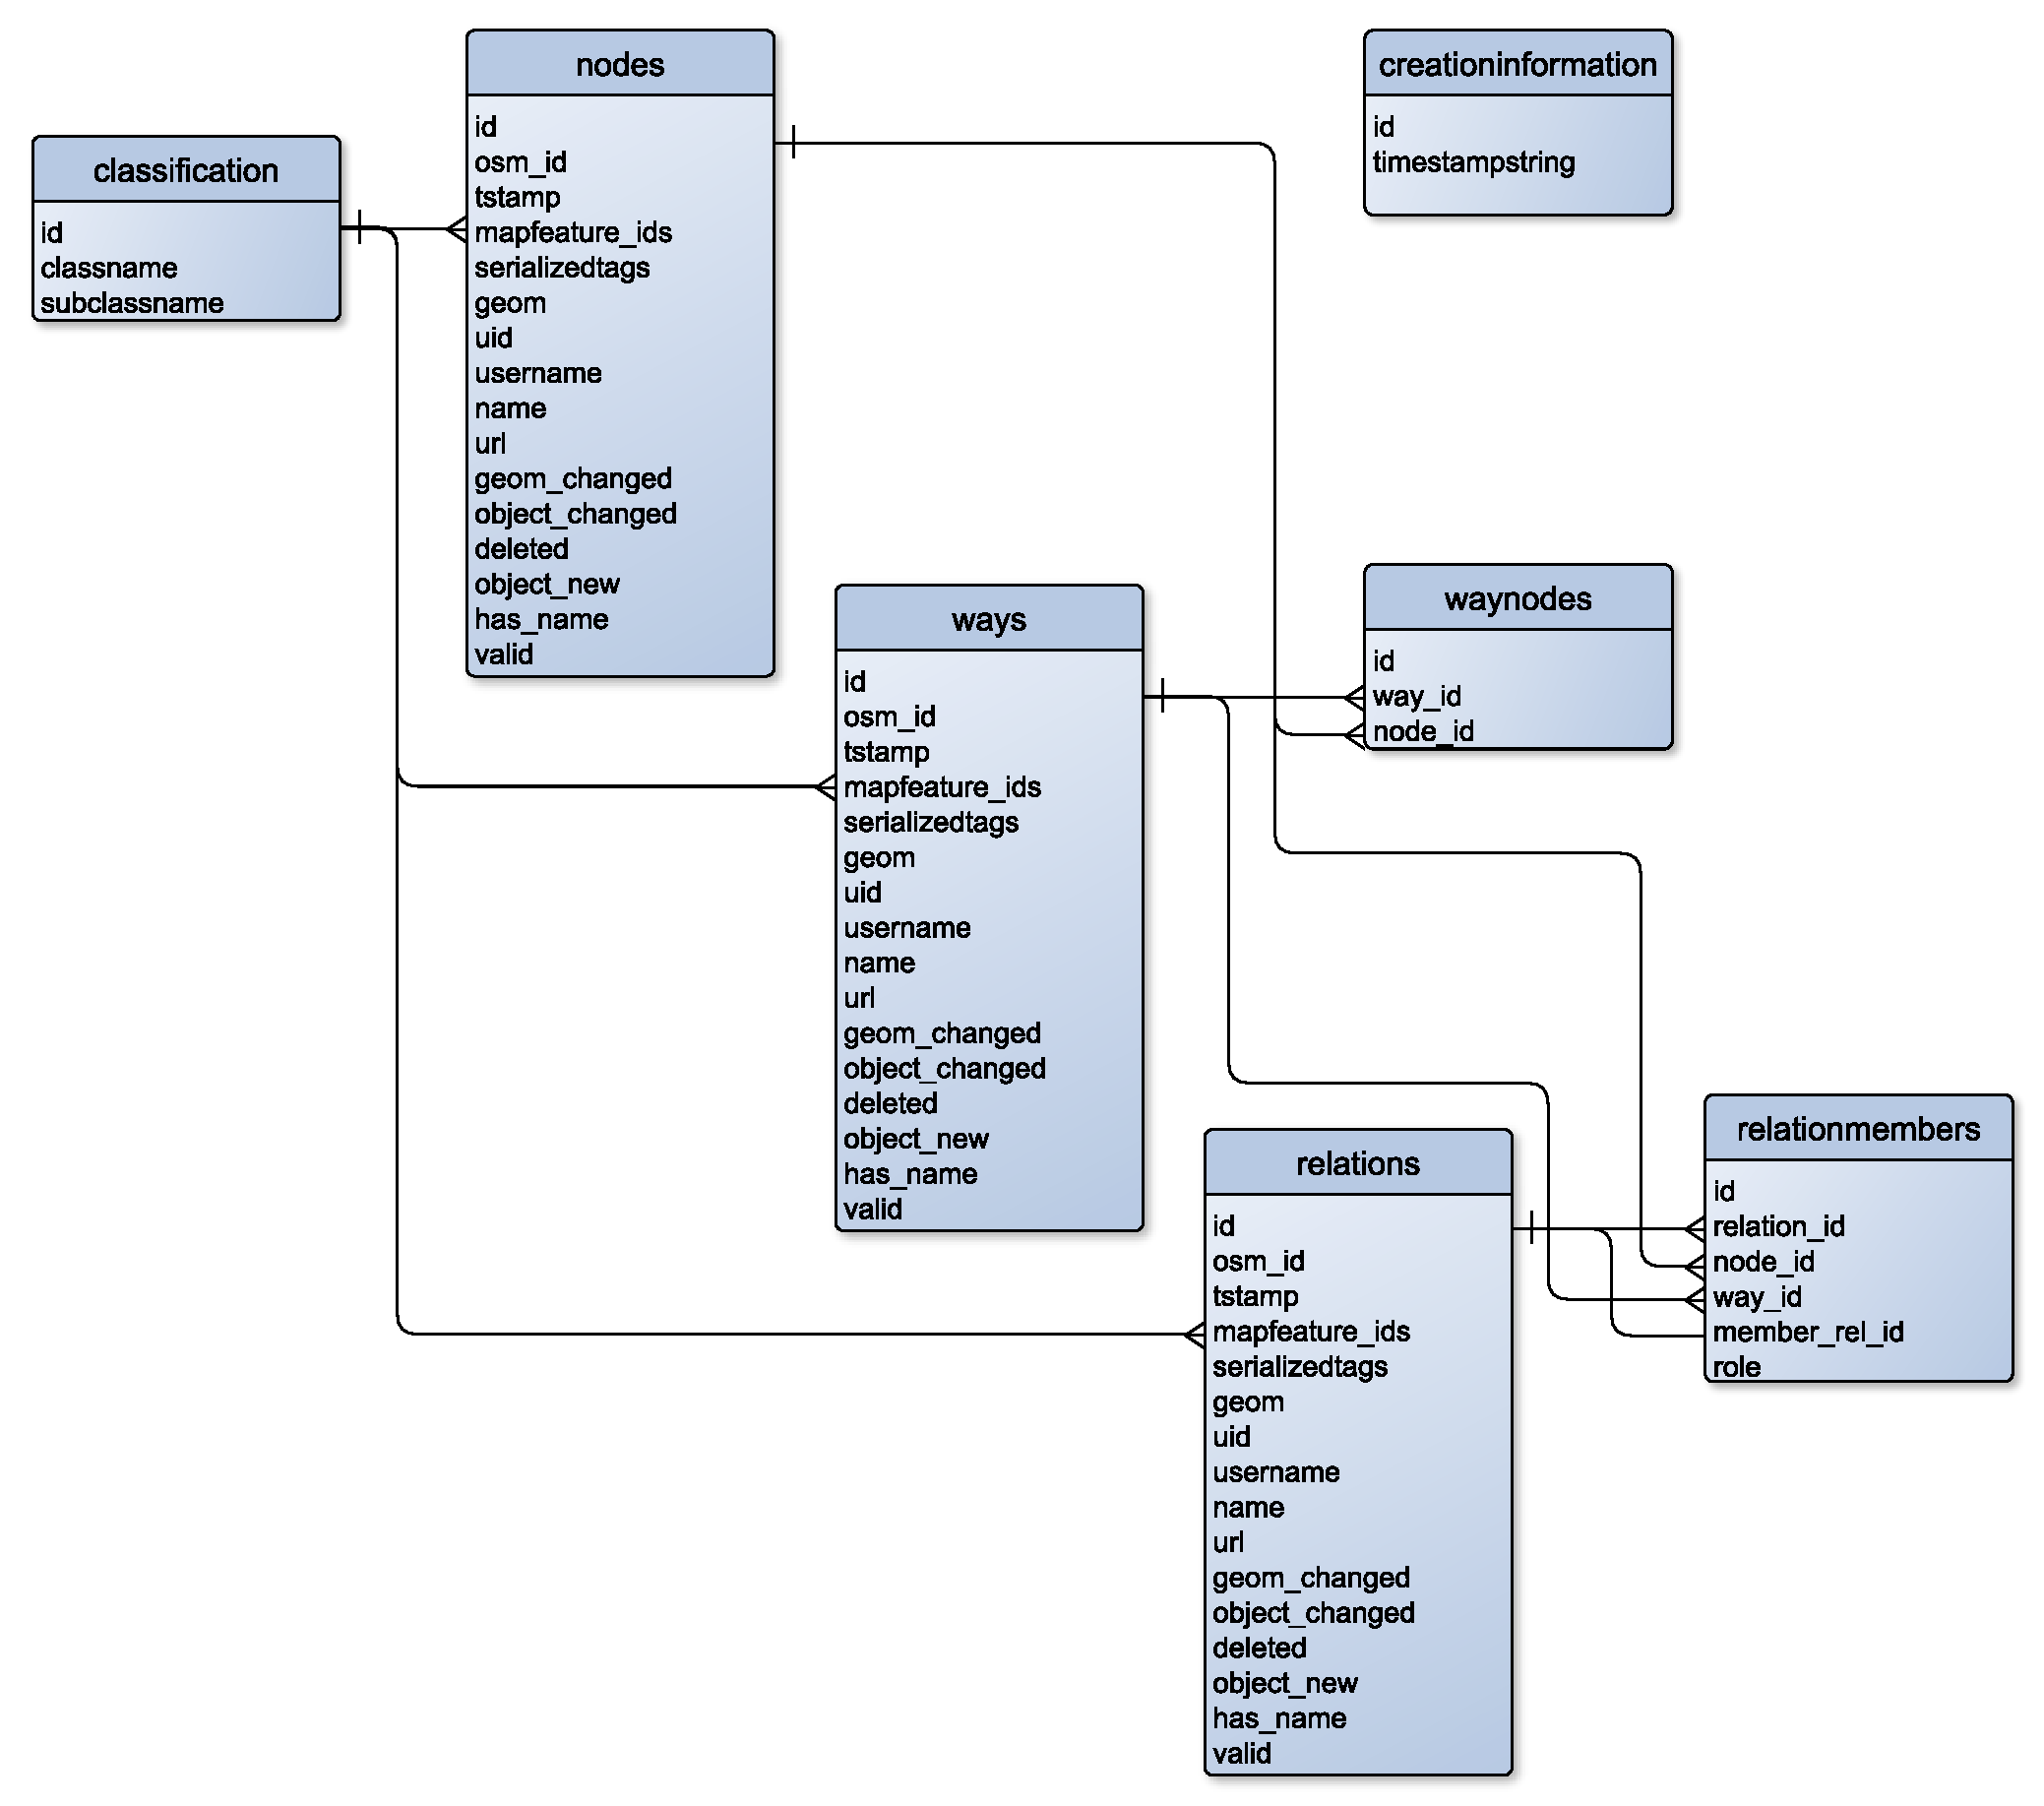
\includegraphics[width=\linewidth]{img/intermediate-db-erd.pdf}
\end{figure}

\newpage
\section{inter2ohdm}
Die Konvertierung der \gls{inter} Datenbank soll mithilfe von SQL Scripts realisiert werden. Hierbei soll, wenn möglich das Tool \gequote{\gls{psql}}\cite{postgres-psql} eingesetzt werden.

\begin{figure}[h]
	\caption{Entity Realtionship Diagramm der \gls{ohdm} Datenbank}
	\label{fig:erd-ohdm}
	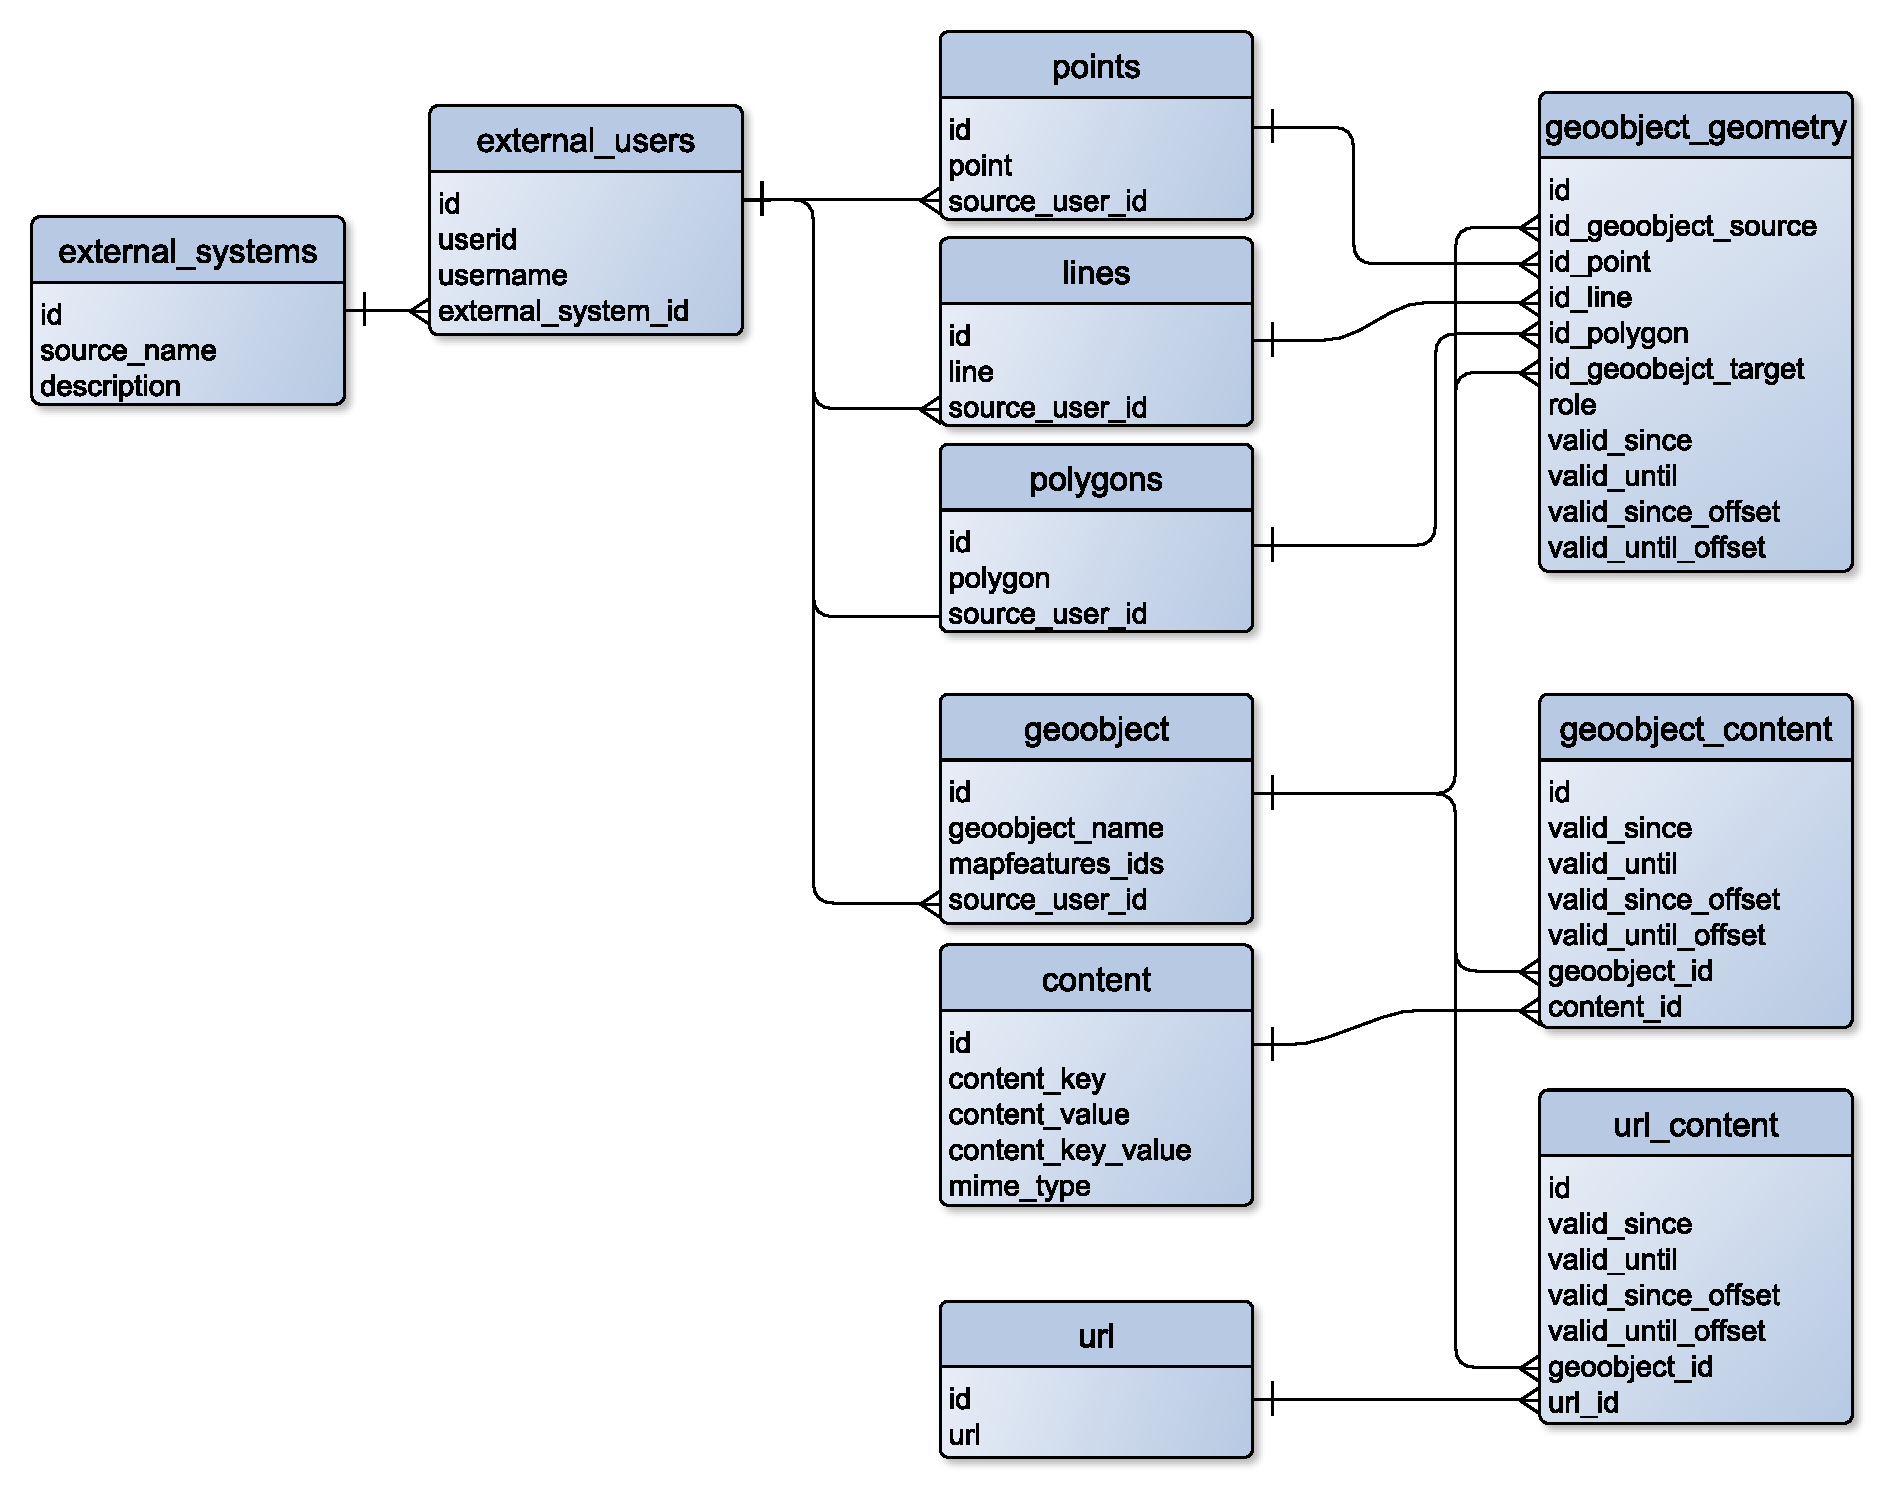
\includegraphics[width=\linewidth]{img/ohdm-db-erd.pdf}
\end{figure}

\section{Zusammenfassung}
Die beiden Datenbankschemata \gls{inter} (vgl. \autoref{fig:erd-inter}) und \gls{ohdm} (vgl. \autoref{fig:erd-ohdm}) sollen beibehalten werden. Allerdings soll jetzt mehr mit den Bordmittel von \gls{osm} und PostgreSQL gearbeitet werden.\\

Die neue Projektidee musste mit bestehenden Datenstrukturen arbeiten, da sonst auch alle anderen Teilprojekte einer Anpassung bedurften.

\chapter{osm2pgsql}
\section{Intro}
Als Importkomponente kann osm2pgsql\cite{osm2pgsql-manual} sehr vielseitig eingesetzt werden. Innerhalb des Projektes löst osm2pgsql den \gls{ohdmconverter} zum importieren von \gls{osm} in die \gls{inter} Datenbank ab. Zusätzlich lassen sich mit dem osm2pgsql nicht nur XML basierte \gls{osm} Dateien importieren sondern auch PBF und BZ2 Container. Allgemein sind \gls{pbf} Datei zu bevorzugen, da sie nur ungefähr halb so groß, wie die XML basierenden \gls{osm} Dateien sind.\cite{osm:pbf}\\

Den größten Vorteil von osm2pgsql bietet die Benutzung des \gequote{\gls{flexoutput}}. Hierbei wird die Konvertierung mit einem Lua Script angepasst.\\

Die Installation kann auf dem GitHub Repository über die \href{https://github.com/OpenHistoricalDataMap/OHDMConverter/tree/SteSad#readme}{Readme.md} eingesehen werden.

\section{osm2pgsql Flags}
Für den fehlerfreien Import sind mehrere Flags notwendig. In der nachfolgenden \autoref{tb:osm2pgsql-flags} sind diese einzeln aufgelistet mit einer entsprechenden Erklärung.
\begin{table}[h]
	\caption{Flags}
	\label{tb:osm2pgsql-flags}
	\renewcommand{\arraystretch}{1.2}
	\begin{tabularx}{\linewidth}{|l|X|}\hline
		\textbf{Flag} & \textbf{Beschreibung}\\\hline
		-H, \texttt{-{}-}host=HOST & Hostname des Datenbankservers oder Standort des Unix-Domänen-Sockets\\\hline
		-P, \texttt{-{}-}port=PORT & Port des Datenbank-Servers\\\hline
		-U, \texttt{-{}-}user=USERNAME & Datenbank-Benutzer\\\hline
		-W, \texttt{-{}-}password & Passwortabfrage erzwingen\\\hline
		-d, \texttt{-{}-}database=DB & Datenbankname oder PostgreSQL Konnektivitätsstring\\\hline
		\texttt{-{}-}log-level=LEVEL & Einstellen der Protokollstufe (debug, info (default), warn, or error)\\\hline
		-x, \texttt{-{}-}extra-attributes & Attribute (Benutzername, Benutzerkennung, Änderungssatzkennung, Zeitstempel und Version) einschließen\\\hline
		-O, \texttt{-{}-}output=OUTPUT & Spezifiziert den Output z.B.: flex, pgsql (Standard), gazetteer und null\\\hline
		-S, \texttt{-{}-}style=STYLE &  Dies gibt an, wie die Daten in die Datenbank importiert werden, ihr Format hängt von der Ausgabe ab.\newline In diesem Flag muss das Lua Script angegeben werden\\\hline		
		-c, \texttt{-{}-}create & Spezifiziert die osm Datei\\\hline
	\end{tabularx}\vspace{0.5cm}
\end{table}

\newpage
\section{Lua Script}
Für den Import in das bestehende \gls{inter} Schema wird ein Lua Script benötigt, welches den Import von \gls{osm} Daten in die \gls{inter} Datenbank spezifiziert.\\
Für eine bessere Erklärung wird das Lua Script in drei Abschnitte unterteilen:
\begin{enumerate}
	\item Tabelleninitialisierung
	\item Hilfsfunktionen und Variablen
	\item Prozessfunktionen
\end{enumerate}
Diese Beschreibung ist projektspezifisch, weitere Informationen zur Verwendung des Lua Script können unter folgendem Link eingesehen werden: \\
\url{https://osm2pgsql.org/doc/manual.html#the-flex-output}
\subsection{Tabelleninitialisierung}\label{subsec:table-init}
Im Lua Script werden erforderliche Tabellen wie in \autoref{lst:table-init-nodes} angelegt. Dies wird benötigt um die Tabelle zu spezifizieren.
\begin{lstlisting}[language={[5.0]Lua}, caption={Initialisierung eine Tabelle für alle nodes},label={lst:table-init-nodes}]
	tables.nodes = osm2pgsql.define_table({
		name = 'nodes',						
		ids = { type = 'node', id_column = 'osm_id' },
		columns = {
			{ column = 'id', sql_type = 'bigserial', create_only = true },
			{ column = 'tstamp', sql_type = 'timestamp' },
			{ column = 'mapfeature_ids', type = 'text' },
			{ column = 'serializedtags', type = 'hstore' },
			{ column = 'geom', type = 'point', projection = 4326 },
			{ column = 'uid', type = 'text' },
			{ column = 'username', type = 'text' },
			{ column = 'name', type = 'text' },
			{ column = 'url', type = 'text' },
			{ column = 'geom_changed', type = 'bool' },
			{ column = 'object_changed', type = 'bool' },
			{ column = 'deleted', type = 'bool' },
			{ column = 'object_new', type = 'bool' },
			{ column = 'has_name', type = 'bool' },
			{ column = 'valid', type = 'bool' }
		},
		schema = SCHEMA_NAME
	})
\end{lstlisting}
\autoref{lst:table-init-nodes} Zeile 4 spezifiziert den osm Typ für den die Tabelle angelegt werden soll (in dem Fall, für alle nodes) und die ID der node wird in die Spalte \gequote{osm\_id} eingetragen.\\
Zeile 6 erzeugt eine Spalte mit einem eindeutigem Integer Wert, welcher mit einem weiteren SQL Script in einen \gequote{Primary Key} verändert werden kann.\\
Die Einträge Zeile 7 - 20 definieren die weiteren Spalten der Tabelle \gequote{nodes}, welche mit einer Prozess Funktion beschrieben werden.\\
Des Weiteren kann wie in Zeile 22 ein Schema definiert werden, in die diese Tabelle geschrieben wird.

\subsection{Hilfsfunktionen und Variablen}
\subsubsection{Map Features}
\begin{lstlisting}[language={[5.0]Lua}, caption={Deklaration einer Lua Tabelle für die mapfeatures},label={lst:table-mapfeatures}]
	local map_features = {
		'admin_level', 'aerialway', 'aeroway', 'amenity', 'barrier', 'boundary',
		'building', 'craft', 'emergency', 'geological', 'healthcare', 'highway',
		'historic', 'landuse', 'leisure', 'man_made', 'military', 'natural',
		'office', 'place', 'power', 'public_transport', 'railway', 'route',
		'shop', 'sport', 'telecom', 'tourism', 'water', 'waterway'
	}
\end{lstlisting}
In \autoref{lst:table-mapfeatures} werden die sogenannten \gequote{\gls{mapfeatures}}\cite{osm-mapfeatures} definiert. \\
OpenStreetMap stellt physische Merkmale am Boden (z. B. Straßen oder Gebäude) mithilfe von Tags dar, die an seine grundlegenden Datenstrukturen (nodes, ways und relations) angehängt sind. Jedes Tag beschreibt ein geografisches Attribut des Features, das von diesem bestimmten nodes, ways oder dieser relations angezeigt wird.\\

Der aktuelle Stand beschriebt zusätzlich im Lua Script eine CSV importiert Tabelle der händisch inserierten Map Features. \\(mehr Ideen: \autoref{ap:ch:curl-mapfeatures})


\subsubsection{Hilfsfunktion für name, mapfeatures, serializedtags und url}\label{subsubsec:get.quadruple}
Die Hilfsfunktion in \autoref{lst:get-quadruple} (nächste Seite) analysiert das übergebene Objekt und gibt vier Werte zurück.
\begin{description}
	\item[name] Der primäre Name: im allgemeinen der prominenteste ausgeschilderte Name oder der gebräuchlichste Name in der/den Landessprache(n). 
	\item[mapfeatures] Eine Lua Tabelle, welche ein key-value Paar enthält. Diese Tabelle enthält alle tags welche eine Übereinstimmung mit der \lstinline|map_features| Lua Tabelle (siehe \autoref{lst:table-mapfeatures}) haben. Der Rückgabetyp ist ein String, der alle IDs der classification Tabelle, Semikolon separiert, enthält.
	\item[serializedtags] Eine Lua Tabelle mit alle object.tags, welche nicht direkt für die weitere Konvertierung benötigt werden.
	\item[url] Bei der Analyse der osm Dateien wurde festgestellt, dass eine url beziehungsweise Websitenreferenz auf verschiedene Arten eingetragen werden kann. Dieses Problem wurde ebenfalls mit der Hilfsfunktion \lstinline| get_tag_quadruple()| realisiert.
\end{description}
Der \textit{goto} Befehl entspricht in diesem Beispiel dem \textit{continue} in Java.\\
Zusätzlich dienen die Zeilen 23 - 42 der Vereinfachung der Tabelleneinträge. Alle Variablen die \lstinline|nil| sind werden in PostgreSQL mit \lstinline|NULL| eingetragen, somit entfällt eine String Vergleich um leere Einträge zu finden. Es kann direkt nach \lstinline|ISNULL| oder \lstinline|NOTNULL| im SQL Statement gefragt werden.

\newpage\begin{lstlisting}[language={[5.0]Lua}, caption={Hilfsfunktion zur osm object.tag Verarbeitung},label={lst:get-quadruple}]
	local function get_tag_quadruple(object)
	-- table with classcodes from the mapfeatures
	local features = {}
	-- declation with one entry '-1' when the osm object has not a mapfeature
	table.insert(features, '-1')
	local ser = {}
	local url = nil
	local name = object:grab_tag('name')
	-- Iterate over each tag from the osm object
	for key, value in pairs(object.tags) do
		-- find url or website entry
		if key == 'url' then
			url = object:grab_tag(key)
			goto continue
		elseif key == 'website' then
			url = object:grab_tag(key)
			goto continue
		elseif osm2pgsql.has_suffix(key, ':url') then
			url = object:grab_tag(key)
			goto continue
		elseif osm2pgsql.has_suffix(key, ':website') then
			url = object:grab_tag(key)
			goto continue
		end
	
		if list_contains(map_features, key) then
			-- osm object.tag is definied as a mapfeature
			features = get_classcode(key, value, features)
			goto continue
		else
			-- osm object.tag is not very relevant,
			-- therefore it is stored in serializedtags table
			ser[key] = value
			goto continue
		end
		:: continue ::
		end
		-- If the table is empty, an empty table should not be saved.
		-- Instead, the value is set to nil (PostgreSQL NULL)
		if next(ser) == nil then
			ser = nil
		end
	-- to save the Lua table as text in PostgreSQL Database,
	-- the table entries concat with ';' as delimiter
	return name, table.concat(features, ';'), url, ser
end
\end{lstlisting}

\newpage
\subsection{Prozessfunktionen}
Damit die nodes, ways, relations spezifisch in die gewünschten Tabellen eingetragen werden, müssen die Lua Funktionen \lstinline|osm2pgsql.process_node| \lstinline|osm2pgsql.process_way| \lstinline|osm2pgsql.process_relation| entsprechend aufgerufen werden. \\
Beispielhaft wurde die definierte Funktion \lstinline|osm2pgsql.process_relation| siehe nächste Seite in \autoref{lst:process-relation} aufgeführt.
Diese enthält:
\begin{table}[h]
	\caption{Kurze Zeilen Beschreibung von \autoref{lst:process-relation}}
	\renewcommand{\arraystretch}{1.2}
	\begin{tabularx}{\linewidth}{|l|l|X|}\hline
		Name & \multirow{2}{*}{\parbox{1.6cm}{Zeilen-\\ nummern}} & Beschreibung\\
		&& \\\hline
		\lstinline|get_tag_quadruple()| & 2 & Erstellung von vier Variablen mit einer Hilfsfunktion (siehe \autoref{subsubsec:get.quadruple})\\\hline
		\lstinline|tables.relations:add_row()| & 3-18 & Fügt ein osm Objekt entsprechend der Tabelleninitialisierung (beispielhaft \autoref{subsec:table-init}) in eine Tabelle ein. \newline Hierbei wird die id automatisch vergeben und eine Geometrie anhand der Bestehenden Daten erzeugt.\\\hline
		Schleife über alle relationmembers & 19-49 & Alle nodes, ways, relations, die im tag \textit{members} vermerkt sind werden in eine seperate Tabelle \textit{relationmembers} eingetragen. Für die Eindeutigkeit wird der Typ des \textit{members} abgefragt. \\\hline
	\end{tabularx}
\end{table}

Die Prozessfunktionen für nodes und ways sieht ähnliches aus, mit dem Unterschied, dass die \lstinline|osm2pgsql.process_node| Funktion keine zusätzlichen \textit{members} besitzt und in \lstinline|osm2pgsql.process_way| die Einträge der ways nur aus nodes bestehen.

\newpage\begin{lstlisting}[language={[5.0]Lua}, caption={Hilfsfunktion zur osm object.tag Verarbeitung},label={lst:process-relation}]
	function osm2pgsql.process_relation(object)
	local object_name, object_features, object_url, object_serializedtags = get_tag_quadruple(object)
	
	tables.relations:add_row({
		name = object_name,
		url = object_url,
		tstamp = reformat_date(object.timestamp),
		mapfeatures = object_features,
		serializedtags = object_serializedtags,
		geom = { create = 'area' },
		uid = object.uid,
		username = object.user,
		geom_changed = false,
		object_changed = false,
		deleted = false,
		object_new = false,
		has_name = false,
		valid = false
	})
	for _, member in ipairs(object.members) do
		-- if type is a node
		if member.type == "n" then
			tables.relationmembers:add_row({
				relation_id = object.id,
				node_id = member.ref,
				way_id = nil,
				member_rel_id = nil,
				role = member.role
			})
		end
		-- if type is a way
		if member.type == "w" then
			tables.relationmembers:add_row({
				relation_id = object.id,
				node_id = nil,
				way_id = member.ref,
				member_rel_id = nil,
				role = member.role
			})
		end
		-- if type is a relation
		if member.type == "r" then
			tables.relationmembers:add_row({
				relation_id = object.id,
				node_id = nil,
				way_id = nil,
				member_rel_id = member.ref,
				role = member.role
			})
		end
	end
end
\end{lstlisting}


\newpage
\section{Ausführung}
Alle vorherigen Sektionen beschreiben die wichtigen Teile des Befehls zum Import von \gls{osm} Daten in die \gls{inter} Datenbank. Der Prozess des Importes kann nun wie folgt ausgeführt werden.
\begin{lstlisting}[language={},basicstyle=\ttfamily,caption={Beispiel eines \gequote{osm2pgsql} Befehls mit dem osm2inter.lua Skript und dem Minimalbeispieldaten littlemap.osm}]
	osm2pgsql \
	--host=localhost \
	--port=5432 \
	--user=postgres \
	--password \
	--database=ohdm \
	--log-level=info \
	--extra-attributes \
	--output=flex \
	--style=/osm2inter/osm2inter.lua \
	--create /osm2inter/littlemap.osm
\end{lstlisting}
\textbf{Hinweis:} Die Dateien müssen mit absoluten Pfaden angegeben werden, oder im Verzeichnis des Datenbanknutzers gespeichert werden.\\

\chapter{psql}
psql ist ein terminalbasiertes Frontend für PostgreSQL. Es ermöglicht Ihnen, Abfragen interaktiv einzugeben, sie an PostgreSQL auszugeben und die Abfrageergebnisse anzuzeigen. Alternativ kann die Eingabe aus einer Datei erfolgen. Darüber hinaus bietet es eine Reihe von Meta-Befehlen und verschiedene shell-ähnliche Funktionen, um das Schreiben von Skripten und die Automatisierung einer Vielzahl von Aufgaben zu erleichtern.\cite{postgres-psql}

Für die Ausführung von psql werden in diesem Beispiel Flags benötigt die in \autoref{tb:psql-flags} aufgeführt sind.
\begin{table}[h]
	\caption{flags}
	\label{tb:psql-flags}
	\renewcommand{\arraystretch}{1.5}
	\begin{tabularx}{\linewidth}{|l|X|}\hline
		\textbf{Flag} & \textbf{Beschreibung}\\\hline
		-H, \texttt{-{}-}host=HOST & Hostname des Datenbankservers oder Standort des Unix-Domänen-Sockets\\\hline
		-P, \texttt{-{}-}port=PORT & Port des Datenbank-Servers\\\hline
		-U, \texttt{-{}-}user=USERNAME & Datenbank-Benutzer\\\hline
		-W, \texttt{-{}-}password & Passwortabfrage erzwingen\\\hline
		-d, \texttt{-{}-}dbname=DB & Datenbankname oder PostgreSQL Konnektivitätsstring\\\hline
		
		-c , \texttt{-{}-}command=command & Spezifiziert den ausführbaren Kommandostring\\\hline
		-f, \texttt{-{}-}file=filename & Ermöglich die Verwendung von Dateien als Quelle für Befehle.\\\hline
	\end{tabularx}\vspace{0.5cm}
\end{table}
\begin{lstlisting}[language={},basicstyle=\ttfamily,caption={Beispiel eines \gequote{psql} Befehls mit dem postprocess.sql Skript}]
	psql \
	--host=localhost \
	--port=5432 \
	--username=postgres \
	--password \
	--dbname=ohdm \
	--file=/osm2inter/osm2inter_postprocess.sql
\end{lstlisting}
\textbf{Hinweis:} Die Dateien müssen mit absoluten Pfaden angegeben werden, oder im Verzeichnis des Datenbanknutzers gespeichert werden.\\

\chapter{OHDM}
Die Konvertierung wird ausschließlich mit einem PostgreSQL Scripts realisiert\footnote{Link zum PostgreSQL Script im OHDMConverter Reporitory\\ \url{https://github.com/OpenHistoricalDataMap/OHDMConverter/blob/SteSad/inter2ohdm/inter2ohdm.sql}}, das mit psql\cite{postgres-psql} gelesen wird. Nachfolgend wird diese Script in drei Teile gesplittet.

\section{Tabellen}
\begin{figure}[h]
	\caption{OHDM Entity Relationship Modell}
	\label{fig:ohdm-erd}
	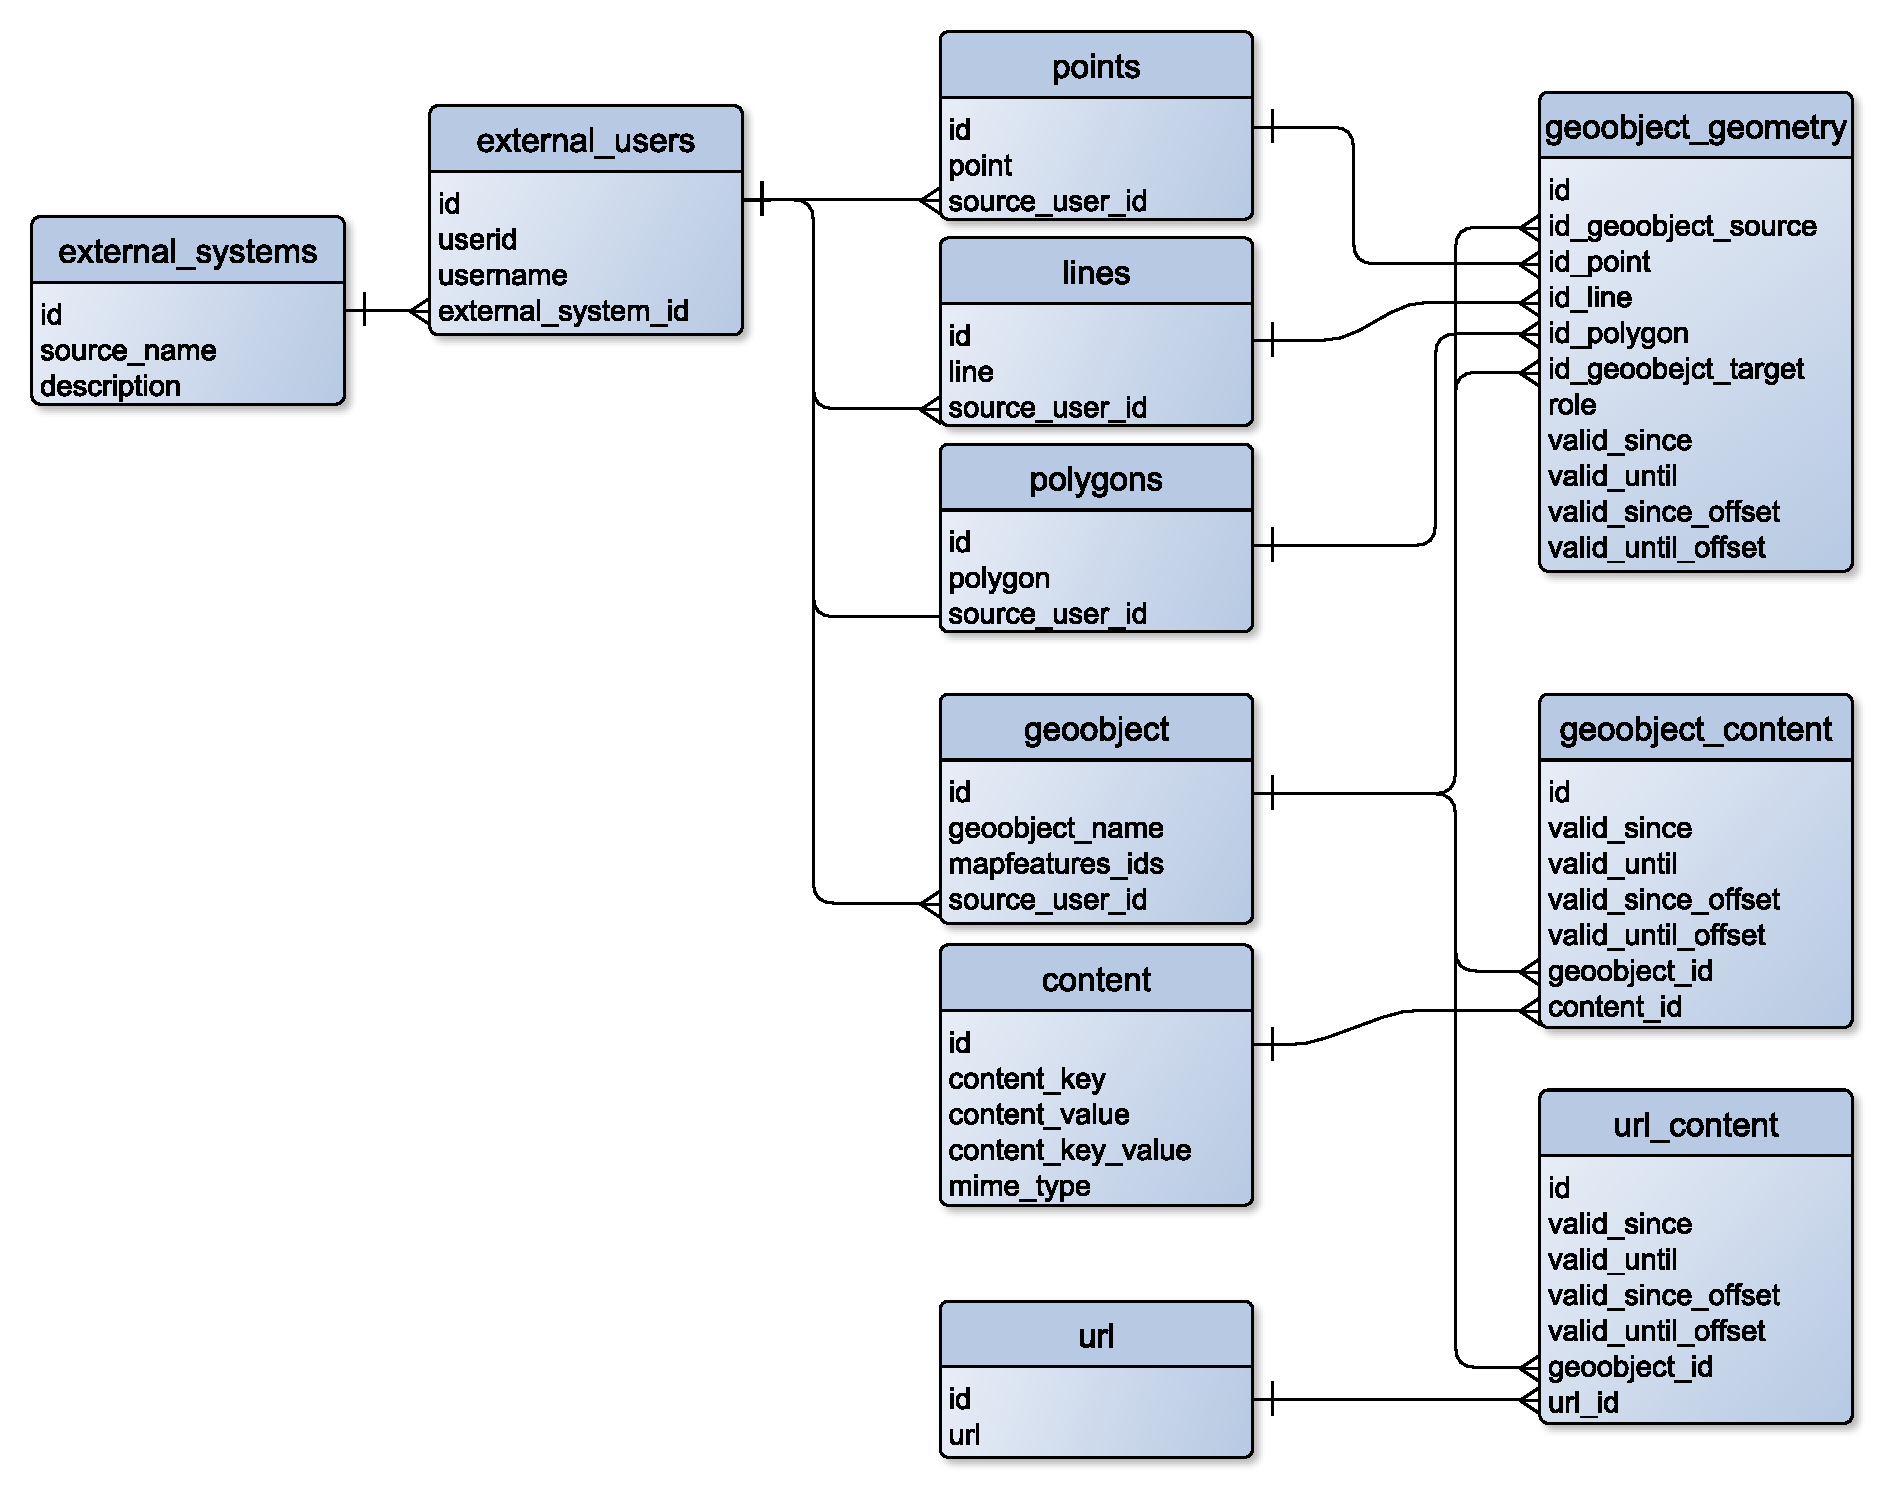
\includegraphics[width=\linewidth]{img/ohdm-db-erd.pdf}
	\caption*{gleich der \autoref{fig:erd-ohdm}}
\end{figure}

Im ersten Teil des PostgreSQL Scriptes werden alle Tabellen (siehe \autoref{fig:ohdm-erd}) erzeugt, die Spaltennamen gesetzt mit deren Datenbankvariablentypen und die Primärschlüssel Eigenschaften eingetragen. Beispielhaft für diesen Vorgang ist in \autoref{lst:sql-create-geoobject-geometry} zu sehen, wie die Tabelle \gequote{geoobject\_geometry} initialisiert wird.\newpage

\begin{lstlisting}[language=SQL,caption={Erzeugung der \gequote{geoobject\_geometry} Tabelle},label={lst:sql-create-geoobject-geometry}]
	CREATE TABLE IF NOT EXISTS ohdm.geoobject_geometry
	(
		id                  BIGSERIAL NOT NULL,
		id_geoobject_source BIGINT,
		id_point            BIGINT,
		id_line             BIGINT,
		id_polygon          BIGINT,
		id_geoobject_target BIGINT,
		role                VARCHAR,
		valid_since         DATE,
		valid_until         DATE,
		valid_since_offset  BIGINT,
		valid_until_offset  BIGINT,
		CONSTRAINT geoobject_geometry_pkey PRIMARY KEY (id)
	);
\end{lstlisting}


\section{Einfacher Insert}
Mehrere Tabellen werden mit simplen SQL Queries initialisiert. Im Beipsiel der Tabelle \gequote{external\_users} werden lediglich die Tabelleneinträge von allen \textit{nodes}, \textit{ways} und \textit{relations} vereinigt. Diese Vereinigungsmenge enthält alle Einträge, die zur Initialisierung der \gequote{external\_users} Tabelle benötigt werden. (vgl. \autoref{lst:insert-users})

\begin{lstlisting}[language=SQL,caption={Insert Statement für die \gequote{external\_users} Tabelle},label={lst:insert-users}]
	INSERT INTO ohdm.external_users(userid, username) 
	(
		SELECT uid::BIGINT, username FROM inter.nodes
		UNION
		SELECT uid::BIGINT, username FROM inter.ways
		UNION
		SELECT uid::BIGINT, username FROM inter.relations
	);
\end{lstlisting}

\newpage
\section{Join Insert}
Die meisten weiteren Initialisierungen werden mithilfe eines JOIN\footnote{vgl. \url{https://www.postgresql.org/docs/current/tutorial-join.html}} Statements realisiert. Hierbei wird eine Vereinigungsmenge gebildet, die abhänig von einer Spalte der beider zu vereinenden Tabellen ist. In \autoref{lst:insert-relation-geometry} wird eine spezielle Initialsiserung aufgezeigt, welche alle Relationen der \gls{inter} Datenbank in Verbindung mit der \gequote{relationmembers} Tabelle in die \gequote{geoobject\_geometry} Tabelle der OHDM Datenbank einfügt.

\begin{lstlisting}[language=SQL,caption={Insert Statement für die \gequote{geoobject\_geometry} Tabelle} auf Basis von allen Realationen der \gls{inter} Datenbank,label={lst:insert-relation-geometry}]
	INSERT INTO ohdm.geoobject_geometry(
		id_geoobject_source, 
		id_polygon, 
		id_geoobject_target, 
		role, 
		valid_since, 
		valid_until
	)
	(
		SELECT source.id, p.id, target.id, rm.role, r.tstamp, CURRENT_TIMESTAMP
		FROM inter.relations AS r
		JOIN inter.relationmembers AS rm ON r.osm_id = rm.relation_id
		JOIN ohdm.geoobject AS source ON r.name = source.geoobject_name
		JOIN ohdm.polygons AS p ON geom = p.polygon
		JOIN inter.relations AS re ON re.osm_id = rm.way_id
		JOIN ohdm.geoobject AS target ON re.name = target.geoobject_name
	);
\end{lstlisting}
	\part{Schlussbetrachtung}
\chapter{Fazit}
Die Implementation des Prototyps ist soweit abgeschlossen, wodurch auch bestehende Tools des OHDMConverters weiterhin das \gls{ohdm} Datenbankschema verwenden können. \\
Im Praktikum wurde viel Wissen erlernt das für den späteren Berufsalltag von Nutzen sein wird:
\begin{itemize}
	\item Der Umgang mit mehreren Komponenten,
	\item Aneignung von Fähigkeiten zur Benutzung von Komponenten durch Lesen der Dokumentationen,
	\item Vertiefung des Wissens im Bereich Datenbank für PostgreSQL,
	\item Umgang mit der Skriptsprache Lua
\end{itemize}

\chapter{Zusätzliche Ergebnisse und Überlegungen}
\section{Laufzeitanalyse}
\begin{table}[h]
	\label{tb:duration}
	\renewcommand{\arraystretch}{1.5}
	\captionsetup{singlelinecheck = false, justification=raggedright}	
	\caption{Laufzeitanalyse}
	\begin{tabular}{|l?r|r|r|r|}\hline
		 Laufzeit & Max & Min & Durchschnitt & Median \\\btrule{1.2pt}
		 Sekunden & 138 & 108 & 128.16 & 128\\\hline
		 Minuten:Sekunden & 02:18 & 01:48 & 02:08 &  02:08\\\hline
	\end{tabular}	
\end{table}

\section{Backgroundprocess}
Im ersten Versuch des Importprozess als Backgroundprocess zu starten wurde folgende Fehlermeldung geloggt.\\
\lstinline[language={}]|sudo: a terminal is required to read the password; either use the -S option to read from standard input or configure an askpass helper|\\
Somit müssen bei dem Backgroundprocess zwei Dinge beachtet werden:
\begin{enumerate}
	\item Die Authentifizierung mit der Datenbank muss per Passwort erfolgen, das heißt dies muss gegebenfalls in der Konfiguration geändert werden.
	\item Der User welcher den Backgroundprocess ausführt muss entsprechende Rechte in der Datenbank besitzen.
	\item psql\cite{postgres-psql} und osm2pgsql\cite{osm2pgsql} müssen mit dem Flag \gequote{-W} ausgeführt werden, um sicherzustellen das die Passworteingabe erfolgen muss.
	\item Das Passwort muss einmalig eingegeben oder zu Ausführung hinterlegt werden.
\end{enumerate}
Hierfür kann ein expect (siehe \autoref{ap:ch:expect}) oder Python Skript geschrieben werden.

\subsection{Python Skript}
Das Python Skript wurde bisher so implementiert, dass ein Datenbankparameter im selben Verzeichnis hinterlegt werden muss. In dieser Datenbankparameter JSON Datei sind alle Parameter der Datenbank, sowie des Nutzers zu vermerken (Beispiel ...)

\begin{lstlisting}[language={},caption={Beispiel einer JSON Datei für die Datenbankparameter}]
	{
		"servername":"localhost",
		"port":"5432",
		"username":"postgres",
		"password":"my_password",
		"database":"ohdm"
	}
\end{lstlisting}
	
	\newpage
\clearscrheadings
\setheadsepline{0px}
\setfootsepline{0px}
\addcontentsline{toc}{chapter}{Quellen}
\chapter*{Quellen}
\section*{Bücher}
\printbibliography[type=book, heading=none]
\section*{Onlinehandbücher}
\printbibliography[type=misc,heading=none]
	%\setcounter{page}{1} \addtocontents{toc}{\protect\pagebreak}
\part{\appendixname}
\appendix
\ihead{\thepart. \parttitle} \chead{} \ohead{\headmark}
\ifoot{\printTitle} \cfoot{Seite \pagemark} \ofoot{}

\newpage
\setheadsepline{.5px}
\setfootsepline{.5px}
\chapter{Multiple Datenbanken in PostgreSQL}\label{ch:clustering}
Die Alternative zur Erstellung eines PostgreSQL Clusters\cite{postgresql-cluster} ist die Verwendung von \lstinline[language=bash]|initdb|\cite{postgresql-cluster}, allerdings gibt mit dieser Variante einige Herausforderungen die mit \lstinline[language=bash]|pg_createcluster| leichter beziehungsweise überhaupt zu bewältigen waren.
\begin{enumerate}
	\item Steuerung des Clusters\cite{postgresql-cluster} für die Serververwaltung
	\item Cluster als Service auch nach einem Neustart des Server starten
\end{enumerate}

\chapter{Curl Map Features}\label{ap:ch:curl-mapfeatures}
Um die Arbeit mit den Map Features\cite{osm-mapfeatures} zu erleichtern, müsste man ein curl Skript implementieren, dass die Tabelleneinträge auf der Map Features\cite{osm-mapfeatures} Webseite ausliest und in eine csv Datei oder ähnliches schreibt.\\

Damit wäre es im Anschluss möglich die csv Datei als Grundlage für ein Insert Statement der classification Tabelle zu verwenden.

\end{document}
